\section{How are we going to archive the goal?}
\subsection{Introduction, Overview}
	To get to our desired goal to have a working scanner that works reliably with a slick GUI, we have to break it down into many smaller goals. Since the scanner will be used to promote the Hochschule, there's some additional steps to cover.
The timeline is as follows:
\begin{itemize}
	\item Build a small rig with 9 cameras to write software and set up the development side of things
	\item Set up all the required servers and development environment:
	\item Set up and automate the (capture and) processing chain/sequence
	\item Design the full scanning array with all 45 SN and lighting
	\item Talk to the workshop people to ensure good design
	\item Build one tower of the final scanning array, 
	\item Calibrate tower (focus, (photogrammetry) settings)
	\item Write software to interface with the lighting system in the tower
	\item Build the remaining towers
	\item Align and calibrate the remaining towers 
	\item Write a GUI to interface with the previous automation scripts or take over the functionality of those entirely. At this point, the scanner is a fully working system
	\item Write additional documentation and Praxissemesterbericht
	\item Render promotional video and art for presentation of the scanner
	\item Work on additional features
\end{itemize}

%% Breakdown of items in sections
\subsection{Software development rig}
	To set up the development environment as well as installing and configuring the required software, a development setup will be built. It consists of
	\begin{itemize}
		\item 9 sensor nodes (SN), each consisting of a Raspberry Pi 4B as a network controller and a camera module V2, with a $8$MP $1/4"$ sensor and $79d$ FOV f/$2$ lens (power is supplied with PoE)
		\item one gigabit network switch, PoE capable to connect the SN with the CN and AS
		\item one compute node (CN) and one array server (AS): AS for controlling the SN and getting the images, CN for calculation of the 3D model from the 2D data - In this setup, CN and AS share the same hardware
	\end{itemize}

	Since it has one CN, one AS, and nine SN, the setup is dubbed \enquote{dev-1-1-9}.	
	
	\begin{figure}[H]
        \centerline{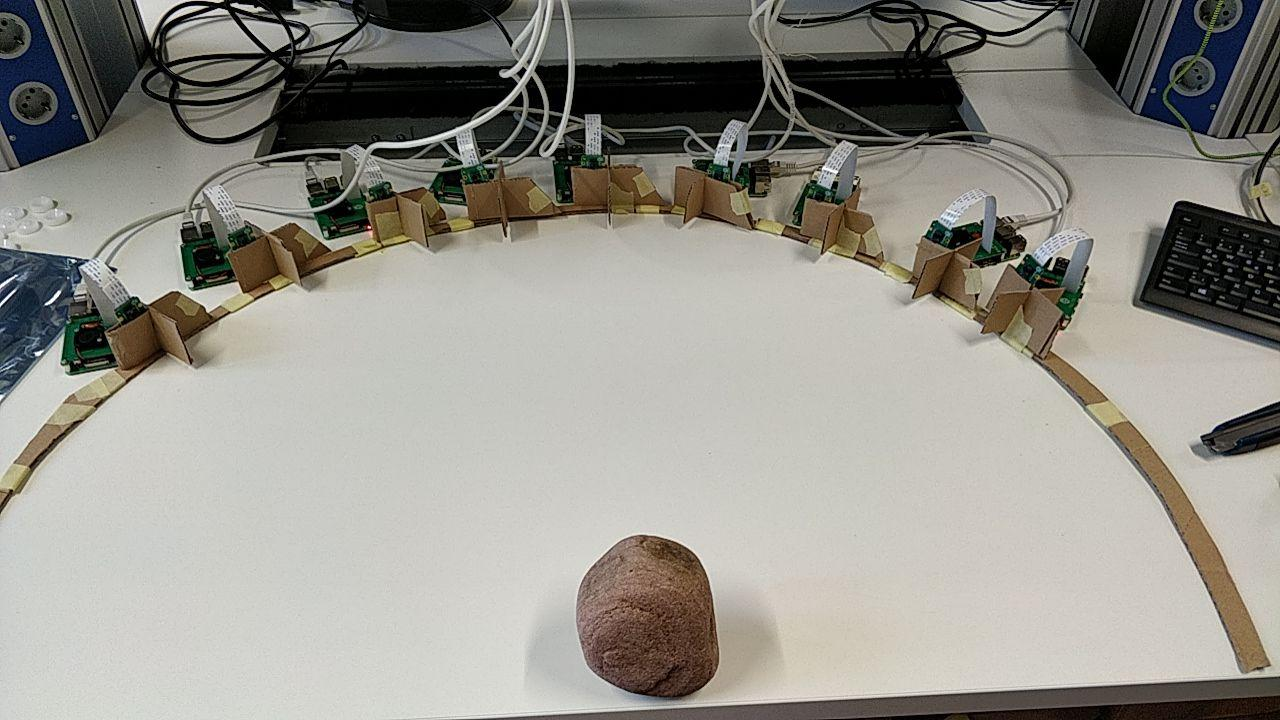
\includegraphics[width=\linewidth]{how/software-devel-rig-1-1-9.jpg}}
        \caption{The software development rig, set up for scanning a stone.}
    \label{software-devel-rig}
    \end{figure}
	
\subsection{Setting up the required software}
	For the scanner to function as such, software has to be set up.
	\begin{itemize}
		\item enabling netboot (PXE) on the SNs by flashing a new bootloader - booting into the SN using an SD card that has the necessary bootloader and a handy script for flashing it
		\item DHCP server on the array server (AS) to assign an IP address to every sensor node when connected to the local network - the built-in DHCP server of DNSMASQ will be used
		\item DHCP client configuration on the SNs - no modification was needed for the Raspberry Pies using Raspberry Pi OS, since the default is to use the IP from DHCP
		\item PXE server and file system on the AS to boot all the SNs from the network, omitting the SD card - the server will be set up using DNSMASQ
		\item NTP server on the AS so that all the SNs share the same time as the AS - this is used for syncronized capture
		\item NTP client configuration on the SNs to get the time from a local time server and not from the web since the SN are not connected to it for security reasons
		\item Compound Pi (CPI) client on the AS to control the cameras on the SN and download the images to the CN - since AS and CN share hardware, the images don't have to be moved from the AS to the CN
		\item CPI server on the SNs to be able to be controlled remotely
		\item enabling SSH on the SN for development and debugging purposes
	\end{itemize}
	
\subsection{Automation of the processing chain}
	The \enquote{Capture and processing sequence}, as seen in figure \ref{operation-flowchart-system}, has to be automated, to later enable operators to use the device \enquote{with the push of a single button}. The automation is split into subsections, to make maintenance and modifications easier. The subsections consist of
	\begin{itemize}
		\item taking all the photos by executing a single script/command
		\item processing photos (built into the chain, but not yet used. Will only be implemented if needed) by executing a single script/command
		\item generating 3D data from photos by executing a single script/command
		\item processing 3D data (same as with photo processing, no 3D processing is done outside of the meshing software, Meshroom) by executing a single script/command
		\item all of the above, but with one command in total
	\end{itemize}
	
	Once that is completed, it is now possible to create a scan with the execution of a single script. Results from the early scans, done by dev-1-1-9, can be seen in figure \ref{stone-mesh} and \ref{face-mesh}.
	
	\begin{figure}[H]
	\centering
	\begin{minipage}{.5\textwidth}
		\centering
    			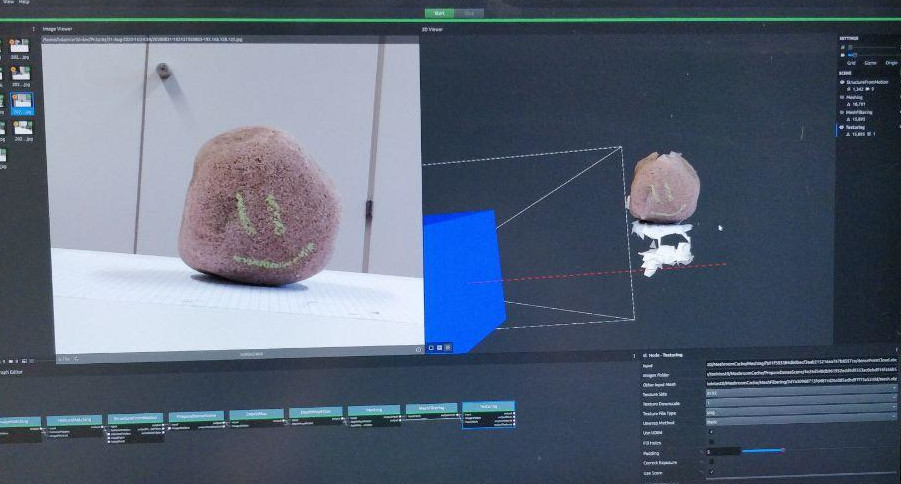
\includegraphics[width=.95\linewidth]{how/stone-meshed.jpg}
    			\captionof{figure}{The stone, meshed using image data from the software development rig.}
    			\label{stone-mesh}
	\end{minipage}%
	\begin{minipage}{.5\textwidth}
		\centering
    			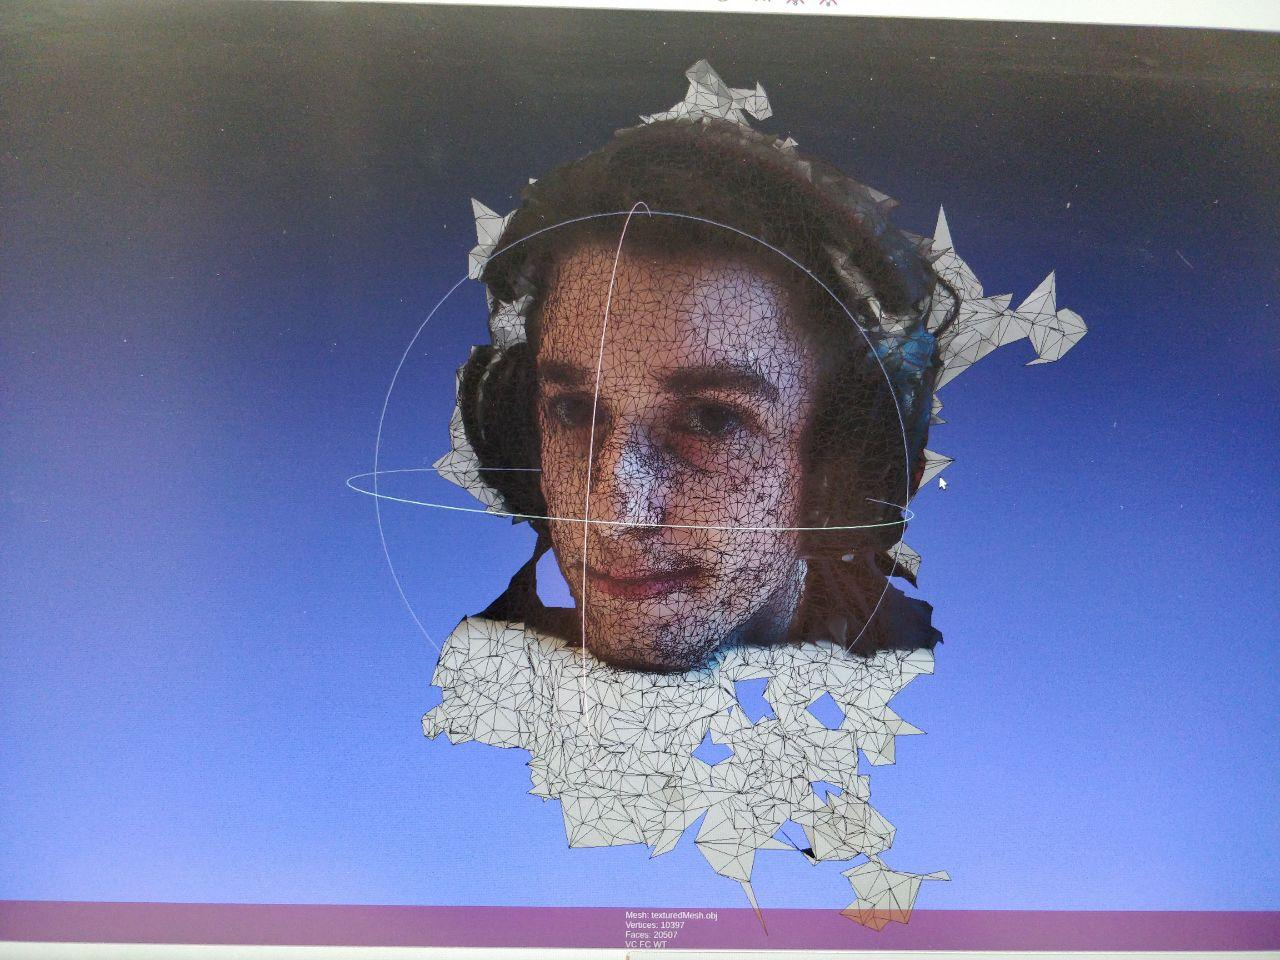
\includegraphics[width=.95\linewidth]{how/headscan-devel-rig.jpg}
	    		\captionof{figure}{My face, meshed using image data from dev-1-1-9.}
	    \label{face-mesh}
		\end{minipage}
	\end{figure}
	
\subsection{Design of the final scanning array with all 45 cameras and lighting}
	Once the software has been set up for the basic operation using a single command, the final scanning array can be designed. There are a number of substeps that go into the design process:
	\begin{itemize}
		\item find out where to place the cameras
		\item find out how many lights are required and where to put them
		\item find out whether LED striplights or spots are more suitable for the job
		\item design a physical construction concept that is
		\begin{itemize}
			\item cheap (after the development setup build, we have $3275.13$\euro{} left from our $5000$\euro{} budget. We need $35$\euro{} more SN at a cost of $52.61$\euro{} each, and we want to build $9$ towers, so the total budget per tower is $160.53$\euro{}, or about $150$\euro{} with an included buffer)
			\item easy to manufacture
			\item solid in the long term (no deformation or degradation that jeopardizes the system integrity)
			\item easy to adjust
			\item easy to maintain
			\item easy to (dis-)assemble once built (array disassembly, for transport)		
			\item portable when split into its modules
		\end{itemize}
	\end{itemize}
	
	\subsubsection{Array layout design}
	To estimate the camera and lighting positions, a simulation was performed using Blender, see figure \ref{blender-sim}. After rendering the $45$ $8MP$ views with $128$ passes and the minimum amount of bounces in Blender - which takes about four hours for a full run on a RTX 2070 using OptiX - the images are loaded into meshroom to recalculate the mesh from the images in high quality. This process takes up to two hours on a Ryzen 5 3600 and an RTX 2070. While lengthy, the simulation helped define the following constraints for the scanning array:
	\begin{itemize}
		\item radius of the scanning circle: $1m$, limited by the space constraints in the lab. A bigger radius means more overlap between images, a smaller radius means more detail but less overlap and possibly problems with too thin of a depth of field. We only have around $45$ cameras to cover a $360d$, $2m$ height cylinder, so we need the overlap for the images to align in the photogrammetry software.
		\item maximum allowed angle between towers to align to the neighboring tower as seen from the center: about $40d$. Smaller angles are better, since there is more overlap in the x-axis of the image. However, since the number of cameras is limited and more towers are more costly, $40d$ was chosen as a sweet spot between tower amounts and tower alignment robustness. The three towers closest to the facial region are only $30d$ apart to increase the camera density and to open the array around back by $20d$ so that entering the array is easier.
		\item camera position and spread across towers: 4-4-5-6-7-6-5-4-4 (9 towers), with the higher amount of cameras in the facial region, and the least amount around the back, since there is less detail in that area compared to the face. The camera and tower position is described in further detail in figure \ref{array-layout-paper}.
		\item camera angle: depending on the camera height. The cameras are angled so that every camera has the most amount of the subject in the frame.
	\end{itemize}
	
	\begin{figure}[H]
        \centerline{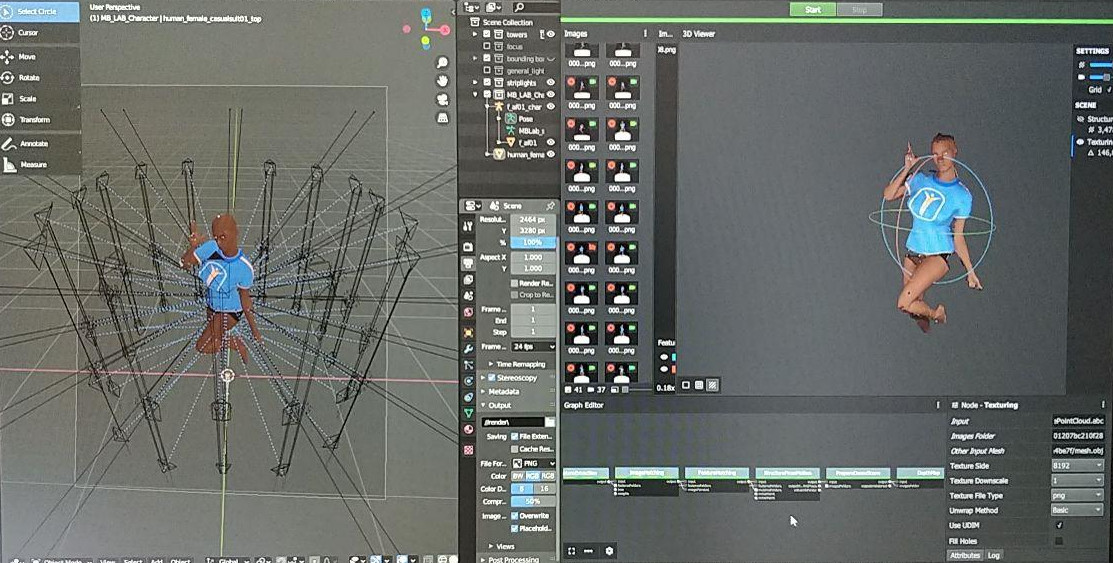
\includegraphics[width=\linewidth]{how/blender-sim.jpg}}
        \caption{Simulation in Blender using 45 cameras and 15 light sources simulating LED strips}
    \label{blender-sim}
    \end{figure}
    
    	\begin{figure}[H]
        \centerline{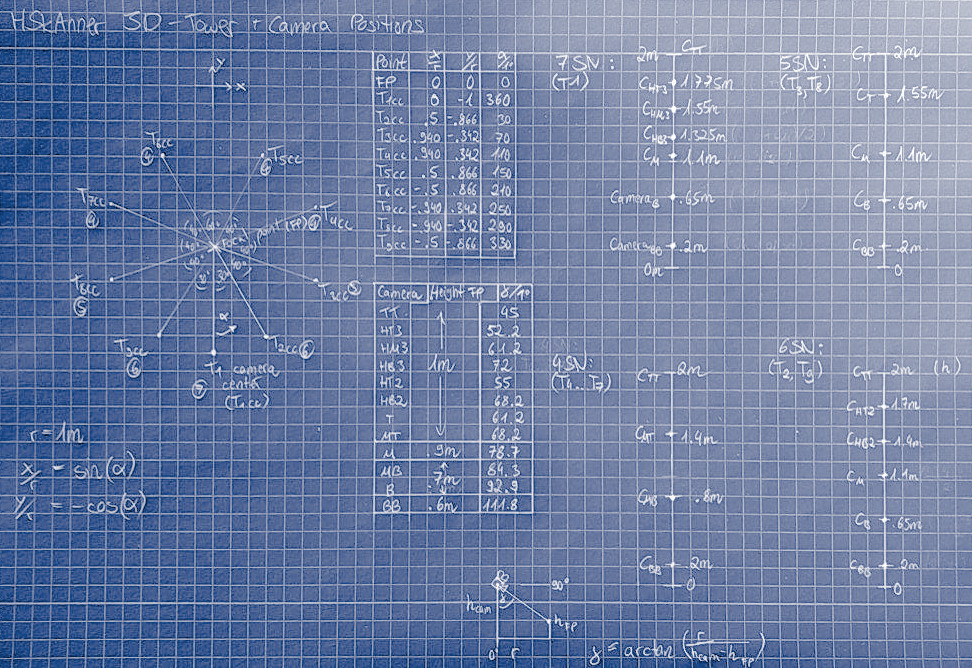
\includegraphics[width=\linewidth]{how/array-layout-paper.jpg}}
        \caption{Final layout and camera angles for the scanning array, estimated using Blender simulation.}
    \label{array-layout-paper}
    \end{figure}
    
    \subsection{Tower design}
	
	
\subsection{Ensuring good physical design}	
	Since mechanical engineering is not my field of expertise, the design of the physical structures will be talked trough with the workshop people to find the correct
	\begin{itemize}
		\item material choice
		\item design for manufacturability
		\item design for CNC machining
	\end{itemize}
	
\subsection{Building one tower}
	After the design has been finalized, parts for one tower will be ordered and it will be assembled. This is done to iron out any mistakes that were overlooked on the hardware or software side, so that the remaining towers can be as good as possible.
	
\subsection{Single tower calibration}
	When the tower has been finished, it will be set up for use and tested. If it passes the test - meaning all cameras align in the photogrammetry software when scanning a human - we can move on. If not, the design will be modified to combat possible shortcomings.
	
\subsection{Lighting control from the AS}
	Once the tower has passed the test, it is time to set up lighting control over the network. This will again be done in steps:
	\begin{itemize}
		\item control the lights using the Raspberry Pi GPIO from the Pi directly
		\item implement functions for fading the lighting in and out as well as RGB effects
		\item set up a (Python?) server on the Pi that is able to control the GPIO and as such can control the lights using the functions or directly writing values
		\item set up a (Python?) client on the AS to send lighting requests to the server on the Pi
		\item integrate lighting control in the automation process
	\end{itemize}
	
\subsection{Building of remaining towers}	
	Now that the towers can be fully controlled, it's time to build the remaining towers and order the rest of the cameras needed.
	
\subsection{Calibration of towers}
	All lenses have to be focused to the middle of the scanner. To do that easily, some setup is required:
	\begin{itemize}
		\item boot the Pies to desktop OS
		\item set up to automatically log in and display camera view once booted
		\item connect an head mounted display (HMD) to HDMI port
		\item focus all cameras manually to central object
	\end{itemize}
	Once the focus is set, the software settings have to be adjusted to the array:
	\begin{itemize}
		\item camera ISO, shutter speed
		\item lighting brightness and fading duration
		\item photogrammetry setting to reliably align the images and get a good quality model as fast as possible
	\end{itemize}

\subsection{GUI for scanner control}
	At this point, all aspects of the scanner have been automated, but the interface is command-line only. A graphical user interface (GUI) is more intuitive for most users and can give quick access to all the required settings and dials of the scanner. It will be created either using Qt (C++) or Tkinter (Python).
	
\subsection{Documentation and Praxissemesterbericht}
	Thus, the scanner as a complete system has been finished. It is possible to change settings from a GUI and a scan can be made with the click of a single button. This marks the start of the documentation and Praxissemesterbericht phase.
	
\subsection{Promotional material}	
	Since the scanner will be used by the Hochschule not only internally but as an attraction on presentation days for the public to see, promotional material will support the concept and add to the experience. I have two concrete ideas:
	\begin{itemize}
		\item a logo for the scanner
		\item a video that will loop on a display near the scanner to show the process from capture to 3D model
	\end{itemize}

\subsection{Additional features}
	To increase the value gained from the setup, additional software features can be developed:
	\begin{itemize}
		\item $360d$ video
		\item motion capture using said video
		\item rendering the 3D model into a scene using e.g. Blender (Mt. Rushmore, ...)
		\item video render of 3D model for viewing pleasure
		\item making the 3D models available from a browser (writing a website, ensuring		 privacy protection)
		\item scanning and meshing improvements, e.g.
			\begin{itemize}
				\item using structured light \cite{meshroom_structlight}
				\item using polarized light
				\item increasing the number of cameras
				\item taking muliple photos in quick succession to increase the effective camera resolution
			\end{itemize}
	\end{itemize}
